\documentclass[12pt,a4paper,twoside,openright,titlepage,final]{article}
\usepackage{fontspec}
\usepackage{amsmath}
\usepackage{amsfonts}
\usepackage{amssymb}
\usepackage{makeidx}
\usepackage{graphicx}
\usepackage[hidelinks,unicode=true]{hyperref}
\usepackage[spanish,es-nodecimaldot,es-lcroman,es-tabla,es-noshorthands]{babel}
\usepackage[left=3cm,right=2cm, bottom=4cm]{geometry}
\usepackage{natbib}
\usepackage{microtype}
\usepackage{ifdraft}
\usepackage{verbatim}
\usepackage[obeyDraft]{todonotes}
\ifdraft{
	\usepackage{draftwatermark}
	\SetWatermarkText{BORRADOR}
	\SetWatermarkScale{0.7}
	\SetWatermarkColor{red}
}{}
\usepackage{booktabs}
\usepackage{longtable}
\usepackage{calc}
\usepackage{array}
\usepackage{caption}
\usepackage{subfigure}
\usepackage{footnote}
\usepackage{url}
\usepackage{tikz}

\setsansfont[Ligatures=TeX]{texgyreadventor}
\setmainfont[Ligatures=TeX]{texgyrepagella}

%*******************************************************
%                 NO MODIFICAR
\newcommand*{\FSfont}[1]{%
  \fontencoding{T1}\fontfamily{#1}\selectfont}

\newlength{\tpheight}\setlength{\tpheight}{0.9\textheight}
\newlength{\txtheight}\setlength{\txtheight}{0.9\tpheight}
\newlength{\tpwidth}\setlength{\tpwidth}{0.9\textwidth}
\newlength{\txtwidth}\setlength{\txtwidth}{0.9\tpwidth}
\newlength{\drop}
%*******************************************************

% Crea una portada con los siguientes parámetros
%
% #1 : Título 
% #2 : Subtítulo
% #3 : Subsubtítulo
% #4 : Autor(es)
% #5 : Lugar
%

\newcommand*{\portada}[5]{
\begin{titlepage}
\begingroup
\vspace*{1cm}
\drop = 0.2\txtheight
\centering
\vfill
{\Huge \scshape #1}\\[\baselineskip]
{\Large \textbf{#2}}\\[\baselineskip]
{\Large \scshape #3}\\[\baselineskip]
\vspace*{0.3cm}
{\large \textit{#4}}\\[0.5\drop]

\includegraphics[scale=0.35]{./imagenes/logoURJC.jpg}
\vspace*{1.5cm}

{\large \scshape #5, \today} \par
\begin{center}
\end{center}
\vfill\null
\endgroup
\end{titlepage}
}
 %*****************************************************
 


\author{José Ignacio Escribano}

\title{Caso práctico II}

\setlength{\parindent}{0pt}

\begin{document}

\pagenumbering{alph}
\setcounter{page}{1}

\portada{Caso Práctico III}{Modelización y tratamiento de la incertidumbre}{Inferencia}{José Ignacio Escribano}{Móstoles}

\listoffigures
\thispagestyle{empty}
\newpage

\tableofcontents
\thispagestyle{empty}
\newpage


\pagenumbering{arabic}
\setcounter{page}{1}

\section{Introducción}

Este caso práctico consta de dos partes relativas a dos modelos distintos: el primero es acerca del modelo beta-binomial, y el segundo, sobre el modelo normal-normal. En ambas partes se piden calcular intervalos de probabilidad y contrastes de hipótesis, entre otras cosas.

\section{Estimando proporciones y predicción de futuras muestras}

En esta primera parte, consideramos una población de 29 niños que tenían un contenido en plomo en los dientes de leche superior a 22.22 partes por millón, de los cuales, 22 terminaron la Educación Secundaria, y 7 que no lo hicieron. Consideraremos que la distribución a priori de la proporción $p$ de niños que terminaron la Educación Secundaria sigue una distribución $p \sim \mathcal{B}e(1,1)$.\\

Lo primero que tenemos que calcular es la función de verosimilitud $\mathcal{L}(p) = P(X = x | p)$. Sabemos que sólo hay dos resultados posibles: terminar o no terminar la Educación Secundaria, por lo que tenemos una distribución binomial con $n = 29$ y $x = 22$.\\

Por tanto, la función de verosimilitud es:

\begin{align*}
\mathcal{L}(p) & = P(X = 22|p) \\ &= \binom{29}{22} p^{22} (1-p)^{29-22} \\ & \propto p^{22} (1-p)^{29-22} \\ & = p^{22}(1-p)^{7}
\end{align*}

Por otro lado, tenemos como distribución a priori una $\mathcal{B}e(1,1)$. La función de densidad de la distribución $\mathcal{B}e(\alpha, \beta)$ viene dada por

\begin{equation*}
f(p|\alpha, \beta) = \begin{cases}
\dfrac{\Gamma(\alpha + \beta)}{\Gamma(\alpha) + \Gamma(\beta)}p^{\alpha - 1}(1-p)^{\beta - 1}, & \text{si } 0 \leq p \leq 1\\
0, & \text{en otro caso} 
\end{cases}
\end{equation*} 

donde $\Gamma(\cdot)$ denota función gamma definida como

\begin{equation*}
\Gamma(x) = \int_{0}^{\infty} t^{x-1}e^{-t} \, dt
\end{equation*}

Por tanto,

\begin{align*}
f(p | \alpha = 1, \beta = 1) & = \dfrac{\Gamma(1 + 1)}{\Gamma(1) + \Gamma(1)}p^{0}(1-p)^{0} \\ & \propto 1 
\end{align*}

Tenemos una distribución a priori que no nos da ninguna información sobre $p$.\\

La distribución a posteriori $f(p|x)$ viene dada por

\begin{align*}
f(p|x) & \propto f(p) \cdot \mathcal{L}(p) \\ & \propto 1 \cdot p^{22}(1-p)^{7} \\ & = p^{22}(1-p)^{7}
\end{align*}

Comparando con la definición de función de densidad de una distribución beta, tenemos que la distribución a posteriori $p|x \sim \mathcal{B}e(23,8)$. Tanto la distribución a posteriori como la distribución empírica son bastante parecidas, por lo que el comando \texttt{rbeta} de R aproxima bien la función aún cunado el número de muestras es relativamente pequeño.\\

La Figura~\ref{fig:distribuciones_beta} muestra las distribuciones a priori, a posteriori y la distribución empírica. Ésta última se ha generado generando con 1000 muestras de una distribución $\mathcal{B}e(23,8)$ (nuestra distribución a posteriori) con el comando \texttt{rbeta} de R. Tanto la distribución beta 
\begin{figure}[tbph!]
\centering
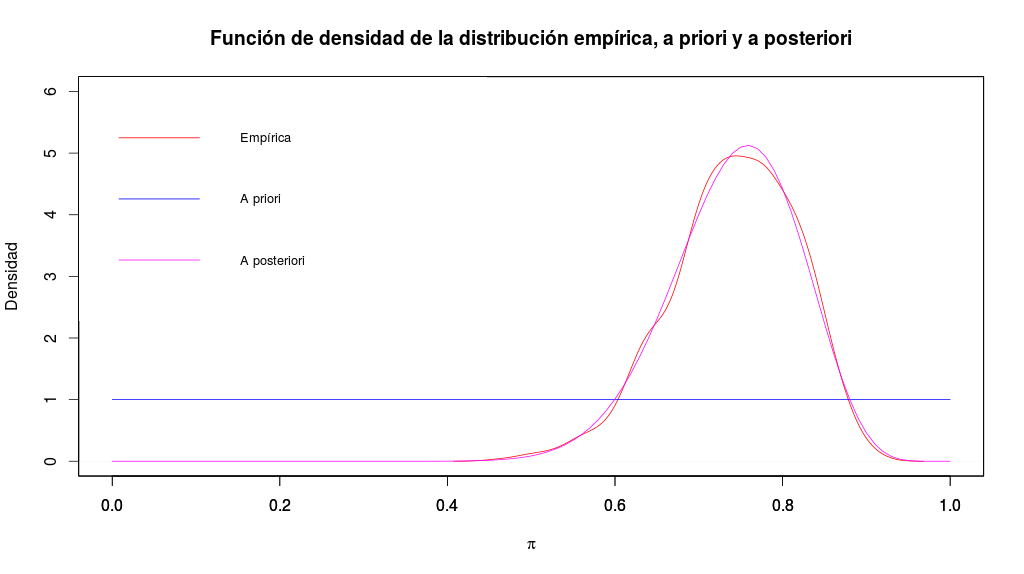
\includegraphics[width=0.9\linewidth]{./imagenes/distribuciones_beta}
\caption{Función de densidad de la distribución empírica, a priori y a posteriori}
\label{fig:distribuciones_beta}
\end{figure}

Como tenemos nuestra distribución a posteriori, podemos calcular la media y la varianza a posteriori de esta distribución, ya que las fórmulas para la media y la varianza son conocidas:

\begin{align*}
E(x|p) & = \dfrac{\alpha}{\alpha + \beta}\\
Var(x|p) & = \dfrac{\alpha \beta}{(\alpha + \beta)^2 (\alpha + \beta + 1)}
\end{align*}

Sustituyendo en las fórmulas anteriores $\alpha$ por 23 y $\beta$ por 8, se tiene que

\begin{align*}
E(x|p) & = 0.7419 \\
Var(x|p) & = 0.0059 \\
\sigma(x|p) & = \sqrt{Var(x|p)} = 0.0773 
\end{align*}


\section{Estimando una media normal con una a priori discreta}

\section{Conclusiones}

\newpage

\section{Código R}

%\verbatiminput{../caso_iii.R}


\end{document} 